% $Id$
\documentclass[a4paper,nologo]{miunart} % students are not allowed to use the
										% university logo
\usepackage[english,swedish]{babel}
\usepackage[utf8]{inputenc}
\usepackage[T1]{fontenc}
\usepackage{natbib}
\usepackage{SIunits}
\usepackage{listings}
\usepackage{varioref,prettyref}
\usepackage{url,hyperref}
\usepackage[varioref,prettyref,natbib,listings]{miunmisc}

\title{Ett exempeldokument för användande av \LaTeX-klassen \texttt{miunart}}
\author{Daniel Bosk\footnote{%
	E-post: \href{mailto:daniel.bosk@miun.se}{daniel.bosk@miun.se}.
	Kurs: DTxxxG Rapportskrivning.
	Handledare: Daniel Bosk.
}}
\date{16 oktober 2012}

\begin{document}
\maketitle
\begin{abstract}
	\noindent
	Ersätt denna text med rapportens sammanfattning.
	Sammanfattningen skall vara kortfattad (högst 200 ord).
	Den skall kunna läsas fristående från resten av rapporten!
	Den får därför inte innehålla några hänvisningar till andra stycken 
	i rapporten.
	Den skall kortfattat beskriva vad som studerats och med vilken metod, samt 
	innehålla viktiga slutsatser som dragits.
	Eventuella mätresultat som anges skall normalt ges med mätosäkerheter.
	Notera att det oftast är enklast att skriva sammanfattningen efter det att 
	man skrivit resten av rapporten.

	\keywords{rapportskrivning, teknik, teknisk rapport}
\end{abstract}


\section{Introduktion}
\label{sec:intro}
\noindent
Ersätt denna text med inledningen.
Inledningen skall klargöra \emph{ämnet} för undersökningen, vad det är för 
\emph{system} som studeras och vilken modell eller vilka modeller som används.
Inledningen bör också ge \emph{nödvändig} bakgrundsinformation relevant för 
förståelsen av undersökningen (vad är känt tidigare; ämnets historik; tidigare 
experimentellt/teoretiskt arbete).
Inledningen skall dessutom beskriva syftet med undersökningen.
I vissa fall kan inledningen inledas med att beskriva syftet, men i andra fall 
behöver viss bakgrundsinformation först ges för att läsaren skall kunna förstå 
vad syftet med undersökningen är.

I slutet av inledningen kan det vara bra att kortfattat beskriva hur resten av 
rapporten är upplagd, det vill säga vad som tas upp i de följande avsnitten.


\section{Teori}
\label{sec:theory}
\noindent
Ersätt denna text med teoriavsnittet.
I de fall då en utförligare beskrivning av den teoretiska modell eller de 
teoretiska modeller som använts är nödvändig bör denna beskrivning göras under 
en egen rubrik.
Teoriavsnittet innehåller principen för modellen/modellerna, definitioner av 
relevanta variabler, den bakomliggande teorin, samt härledning av de ekvationer 
som använts.
Mycket långa härledningar kan redovisas i bilaga.

Centrala samband/ekvationer numreras och anges på egen rad.
Se exempelvis
\begin{equation}
	\label{eq:long-equation}
	y = y_0 + v_{y_0}t + \frac{1}{2}a_yt^2,
\end{equation}
där \(y\) är ett samband som beror av hastigheten \(v\), en faktor \(a\) och 
tiden \(t\).
(Dessa ska naturligtvis förklaras bättre i en skarp text.)

Vid hänvisning till ekvationen används numreringen, exempelvis 
utgångshastigheten \(v_{y_0}\) i ekvation \prettyref{eq:long-equation}.


\section{Metod}
\label{sec:method}
\noindent
En alternativ rubrik är \emph{Modell}.
Är det ett experimentellt arbete så kan även \emph{Experiment} användas som 
rubrik.

\begin{figure}
	\centering
	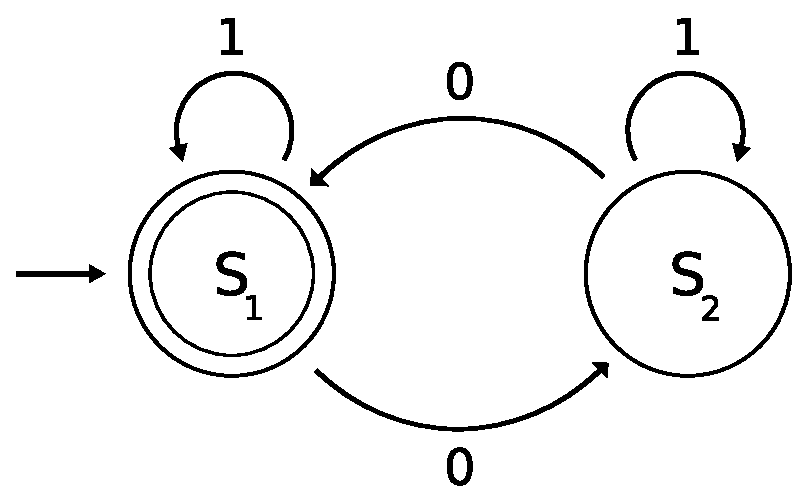
\includegraphics[width=0.7\linewidth]{automata.eps}
	\caption{Ett exempel på den abstrakta datastrukturen automat.}
	\label{fig:automata}
\end{figure}

Avsnittet bör inledas med en övergripande beskrivning av vad som har mätits 
eller beräknats.
Efter den övergripande beskrivningen följer en mer detaljerad beskrivning av 
hur mätningar eller beräkningar av de kvantiteter som är nödvändiga att 
bestämma gjordes och med vilken utrustning, beskriv också eventuell 
provpreparering eller andra steg som togs i experimentet.
I många fall är det lämpligt att beskriva experimentuppställningen med en 
schematisk skiss.
I vissa fall kan experimentuppställningen vara så komplicerad eller så viktig 
att den beskrivs under egen rubrik.
Rubriken \emph{Experimentuppställning} placeras då lämpligen innan 
metodavsnittet.

Eventuella bilder infogas.
Se exempelvis \prettyref{fig:automata}.
Exempelvis skulle hänvisningen i detta fall kunna inledas med 
i \prettyref{fig:automata} visas en schematisk bild av experimentuppställningen 
vid försöket.


\section{Resultat och diskussion}
\label{sec:results}
\noindent
Ersätt denna text.
I en kortare rapport kan det vara lämpligt att slå ihop resultatavsnittet med 
diskussionsavsnittet under en rubrik.
Blir avsnitten långa är det dock lämpligt att dela upp dessa avsnitt under två 
rubriker.

Vanligtvis används de uppmätta värdena för att beräkna någon eller några andra 
storheter.
Det beräknade resultatet kan exempelvis vara lutningen i en graf eller på annat 
sätt beräknat från de uppmätta värdena.
Ange hur det beräknade värdet (eller beräknade värdena) har bestämts från de 
uppmätta värdena.
Redovisa vidare hur mätosäkerheten i slutresultatet har beräknats/uppskattats.
Längre beräkningar av mätosäkerhet placeras lämpligen i en bilaga (med 
hänvisning till bilagan i texten), eller under egen rubrik i de fall då 
uppskattning av mätosäkerheten är en central del av syftet med undersökningen.

\begin{table}
	\centering
	\begin{tabular}{ccc}
		\hline\hline
		\textbf{Höjd, \(h\) (\metre) \(\pm\) \unit{0.01}{\metre}} &
		\textbf{Tid, \(t\) (\second)} &
		\textbf{Mätosäkerhet i tiden, \(u(t)\) (\second)} \\
		\hline
		0.86 &	0.38 &	0.06 \\
		2.02 &	0.65 &	0.06 \\
		3.01 &	0.79 &	0.10 \\
		4.26 &	0.99 &	0.10 \\
		\hline\hline
	\end{tabular}
	\caption{Falltid för en kula från olika höjder.}
	\label{tab:kula}
\end{table}

Ett exempel på en tabell återfinns i \prettyref{tab:kula}.
Ge en kortfattad text som beskriver vad tabellen innehåller som tabelltext.
Ange storhet och enhet i tabellhuvud.
%Mätvärdena bör justeras så att decimalkommana hamnar under varandra.
Ange mätvärdena med så många värdesiffror som motiveras av mätosäkerheten, det 
vill säga osäkerheten skall ligga i den sista siffran.
Mätosäkerheten skall aldrig ges med fler än två värdesiffror!
Ange gärna mätosäkerheterna i tabellen, som i exemplet ovan.
Använd prefix eller tiopotenser framför enheterna i tabellhuvudet för att göra 
värdena i tabellen lättlästa.

När ni gör diagram bör ni tänka på ett antal saker.
För dessa används figurer.
Figuren skall innehålla en förklarande figurtext.
Axlarna i diagrammet skall innehålla axelrubriker med korrekta enheter.
Skalan på axlarna skall vara tydligt markerad.
Mätpunkterna skall markeras med stora tydliga symboler.
Om det behövs för tolkningen av resultatet skall en \emph{bästa anpassning}
ritas in.
Anpassa skalan på axlarna så att figuren blir tydlig.
Det kan till exempel innebära att en logaritmisk skala används på en eller båda 
axlarna.
I regel bör axlarna väljas så att en sökt storhet kan fås från till exempel 
lutningen av en anpassad rät linje.

Diskussionsavsnittet skall innehålla en tolkning av resultaten.
Har några begränsningar i metoden upptäckts?
Stödjer data antagna hypoteser?
Om de inte gör det, vad kan det bero på?
De viktigaste detaljerna som framkommit i studien bör belysas i diskussionen.

I en kortare rapport kan det vara naturligt att varva resultat med diskussion 
av resultaten, istället för att ge dessa i två separata avsnitt.


\section{Slutsatser}
\label{sec:conclusion}
\noindent
I detta avsnitt återkommer man till syftet med experimentet/studien.
Vad var syftet med studien och hur väl uppnåddes målen med studien.
Här sammanfattar du dina resultat av mätningarna, presenterar de viktigaste 
slutsatserna (från diskussionen) och anger eventuella viktiga slutresultat med 
mätosäkerheter (om sådana bestämts).

Här gör man också gärna jämförelser mellan föreliggande arbete och tidigare 
arbeten -- glöm inte att ge källreferens till tidigare arbeten, exempelvis 
\cite{Knuth1989arr}.
Idéer till förbättringar och fortsatt arbete kan också beskrivas här.


\bibliography{example}
\end{document}
